% Created by tikzDevice version 0.12
% !TEX encoding = UTF-8 Unicode
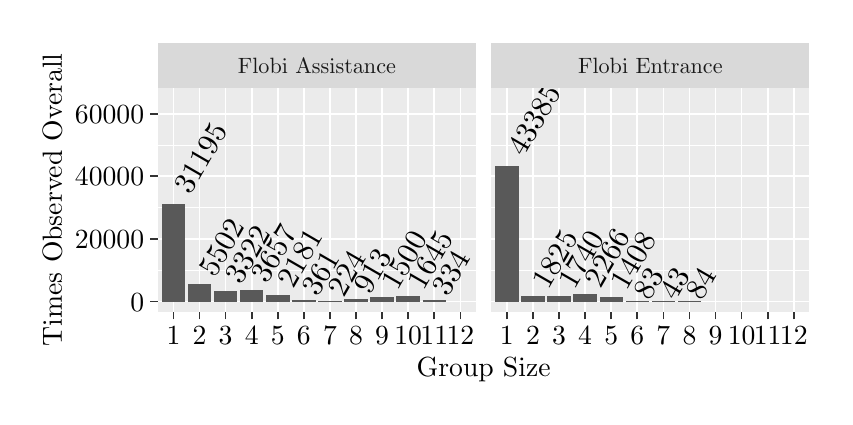
\begin{tikzpicture}[x=1pt,y=1pt]
\definecolor{fillColor}{RGB}{255,255,255}
\path[use as bounding box,fill=fillColor,fill opacity=0.00] (0,0) rectangle (288.00,133.49);
\begin{scope}
\path[clip] (  0.00,  0.00) rectangle (288.00,133.49);
\definecolor{drawColor}{RGB}{255,255,255}
\definecolor{fillColor}{RGB}{255,255,255}

\path[draw=drawColor,line width= 0.6pt,line join=round,line cap=round,fill=fillColor] (  0.00,  0.00) rectangle (288.00,133.49);
\end{scope}
\begin{scope}
\path[clip] ( 47.03, 30.86) rectangle (162.01,111.73);
\definecolor{fillColor}{gray}{0.92}

\path[fill=fillColor] ( 47.03, 30.86) rectangle (162.01,111.73);
\definecolor{drawColor}{RGB}{255,255,255}

\path[draw=drawColor,line width= 0.3pt,line join=round] ( 47.03, 45.85) --
	(162.01, 45.85);

\path[draw=drawColor,line width= 0.3pt,line join=round] ( 47.03, 68.47) --
	(162.01, 68.47);

\path[draw=drawColor,line width= 0.3pt,line join=round] ( 47.03, 91.09) --
	(162.01, 91.09);

\path[draw=drawColor,line width= 0.6pt,line join=round] ( 47.03, 34.54) --
	(162.01, 34.54);

\path[draw=drawColor,line width= 0.6pt,line join=round] ( 47.03, 57.16) --
	(162.01, 57.16);

\path[draw=drawColor,line width= 0.6pt,line join=round] ( 47.03, 79.78) --
	(162.01, 79.78);

\path[draw=drawColor,line width= 0.6pt,line join=round] ( 47.03,102.40) --
	(162.01,102.40);

\path[draw=drawColor,line width= 0.6pt,line join=round] ( 52.68, 30.86) --
	( 52.68,111.73);

\path[draw=drawColor,line width= 0.6pt,line join=round] ( 62.11, 30.86) --
	( 62.11,111.73);

\path[draw=drawColor,line width= 0.6pt,line join=round] ( 71.53, 30.86) --
	( 71.53,111.73);

\path[draw=drawColor,line width= 0.6pt,line join=round] ( 80.96, 30.86) --
	( 80.96,111.73);

\path[draw=drawColor,line width= 0.6pt,line join=round] ( 90.38, 30.86) --
	( 90.38,111.73);

\path[draw=drawColor,line width= 0.6pt,line join=round] ( 99.81, 30.86) --
	( 99.81,111.73);

\path[draw=drawColor,line width= 0.6pt,line join=round] (109.23, 30.86) --
	(109.23,111.73);

\path[draw=drawColor,line width= 0.6pt,line join=round] (118.66, 30.86) --
	(118.66,111.73);

\path[draw=drawColor,line width= 0.6pt,line join=round] (128.08, 30.86) --
	(128.08,111.73);

\path[draw=drawColor,line width= 0.6pt,line join=round] (137.51, 30.86) --
	(137.51,111.73);

\path[draw=drawColor,line width= 0.6pt,line join=round] (146.93, 30.86) --
	(146.93,111.73);

\path[draw=drawColor,line width= 0.6pt,line join=round] (156.36, 30.86) --
	(156.36,111.73);
\definecolor{fillColor}{gray}{0.35}

\path[fill=fillColor] ( 48.44, 34.54) rectangle ( 56.92, 69.82);

\path[fill=fillColor] ( 57.86, 34.54) rectangle ( 66.35, 40.76);

\path[fill=fillColor] ( 67.29, 34.54) rectangle ( 75.77, 38.30);

\path[fill=fillColor] ( 76.71, 34.54) rectangle ( 85.20, 38.67);

\path[fill=fillColor] ( 86.14, 34.54) rectangle ( 94.62, 37.01);

\path[fill=fillColor] ( 95.56, 34.54) rectangle (104.05, 34.95);

\path[fill=fillColor] (104.99, 34.54) rectangle (113.47, 34.79);

\path[fill=fillColor] (114.42, 34.54) rectangle (122.90, 35.57);

\path[fill=fillColor] (123.84, 34.54) rectangle (132.32, 36.23);

\path[fill=fillColor] (133.27, 34.54) rectangle (141.75, 36.40);

\path[fill=fillColor] (142.69, 34.54) rectangle (151.17, 34.92);
\definecolor{drawColor}{RGB}{0,0,0}

\node[text=drawColor,rotate= 60.00,anchor=base west,inner sep=0pt, outer sep=0pt, scale=  1.10] at ( 58.73, 72.70) {31195};

\node[text=drawColor,rotate= 60.00,anchor=base west,inner sep=0pt, outer sep=0pt, scale=  1.10] at ( 67.61, 42.68) {5502};

\node[text=drawColor,rotate= 60.00,anchor=base west,inner sep=0pt, outer sep=0pt, scale=  1.10] at ( 77.03, 40.22) {3322};

\node[text=drawColor,rotate= 60.00,anchor=base west,inner sep=0pt, outer sep=0pt, scale=  1.10] at ( 86.46, 40.60) {3657};

\node[text=drawColor,rotate= 60.00,anchor=base west,inner sep=0pt, outer sep=0pt, scale=  1.10] at ( 95.88, 38.93) {2181};

\node[text=drawColor,rotate= 60.00,anchor=base west,inner sep=0pt, outer sep=0pt, scale=  1.10] at (104.75, 35.91) {361};

\node[text=drawColor,rotate= 60.00,anchor=base west,inner sep=0pt, outer sep=0pt, scale=  1.10] at (114.18, 35.76) {224};

\node[text=drawColor,rotate= 60.00,anchor=base west,inner sep=0pt, outer sep=0pt, scale=  1.10] at (123.60, 36.54) {913};

\node[text=drawColor,rotate= 60.00,anchor=base west,inner sep=0pt, outer sep=0pt, scale=  1.10] at (133.58, 38.16) {1500};

\node[text=drawColor,rotate= 60.00,anchor=base west,inner sep=0pt, outer sep=0pt, scale=  1.10] at (143.01, 38.32) {1645};

\node[text=drawColor,rotate= 60.00,anchor=base west,inner sep=0pt, outer sep=0pt, scale=  1.10] at (151.88, 35.88) {334};
\end{scope}
\begin{scope}
\path[clip] (167.51, 30.86) rectangle (282.50,111.73);
\definecolor{fillColor}{gray}{0.92}

\path[fill=fillColor] (167.51, 30.86) rectangle (282.50,111.73);
\definecolor{drawColor}{RGB}{255,255,255}

\path[draw=drawColor,line width= 0.3pt,line join=round] (167.51, 45.85) --
	(282.50, 45.85);

\path[draw=drawColor,line width= 0.3pt,line join=round] (167.51, 68.47) --
	(282.50, 68.47);

\path[draw=drawColor,line width= 0.3pt,line join=round] (167.51, 91.09) --
	(282.50, 91.09);

\path[draw=drawColor,line width= 0.6pt,line join=round] (167.51, 34.54) --
	(282.50, 34.54);

\path[draw=drawColor,line width= 0.6pt,line join=round] (167.51, 57.16) --
	(282.50, 57.16);

\path[draw=drawColor,line width= 0.6pt,line join=round] (167.51, 79.78) --
	(282.50, 79.78);

\path[draw=drawColor,line width= 0.6pt,line join=round] (167.51,102.40) --
	(282.50,102.40);

\path[draw=drawColor,line width= 0.6pt,line join=round] (173.17, 30.86) --
	(173.17,111.73);

\path[draw=drawColor,line width= 0.6pt,line join=round] (182.59, 30.86) --
	(182.59,111.73);

\path[draw=drawColor,line width= 0.6pt,line join=round] (192.02, 30.86) --
	(192.02,111.73);

\path[draw=drawColor,line width= 0.6pt,line join=round] (201.44, 30.86) --
	(201.44,111.73);

\path[draw=drawColor,line width= 0.6pt,line join=round] (210.87, 30.86) --
	(210.87,111.73);

\path[draw=drawColor,line width= 0.6pt,line join=round] (220.29, 30.86) --
	(220.29,111.73);

\path[draw=drawColor,line width= 0.6pt,line join=round] (229.72, 30.86) --
	(229.72,111.73);

\path[draw=drawColor,line width= 0.6pt,line join=round] (239.14, 30.86) --
	(239.14,111.73);

\path[draw=drawColor,line width= 0.6pt,line join=round] (248.57, 30.86) --
	(248.57,111.73);

\path[draw=drawColor,line width= 0.6pt,line join=round] (257.99, 30.86) --
	(257.99,111.73);

\path[draw=drawColor,line width= 0.6pt,line join=round] (267.42, 30.86) --
	(267.42,111.73);

\path[draw=drawColor,line width= 0.6pt,line join=round] (276.84, 30.86) --
	(276.84,111.73);
\definecolor{fillColor}{gray}{0.35}

\path[fill=fillColor] (168.93, 34.54) rectangle (177.41, 83.61);

\path[fill=fillColor] (178.35, 34.54) rectangle (186.83, 36.60);

\path[fill=fillColor] (187.78, 34.54) rectangle (196.26, 36.51);

\path[fill=fillColor] (197.20, 34.54) rectangle (205.68, 37.10);

\path[fill=fillColor] (206.63, 34.54) rectangle (215.11, 36.13);

\path[fill=fillColor] (216.05, 34.54) rectangle (224.54, 34.63);

\path[fill=fillColor] (225.48, 34.54) rectangle (233.96, 34.59);

\path[fill=fillColor] (234.90, 34.54) rectangle (243.39, 34.63);
\definecolor{drawColor}{RGB}{0,0,0}

\node[text=drawColor,rotate= 60.00,anchor=base west,inner sep=0pt, outer sep=0pt, scale=  1.10] at (179.22, 86.49) {43385};

\node[text=drawColor,rotate= 60.00,anchor=base west,inner sep=0pt, outer sep=0pt, scale=  1.10] at (188.09, 38.53) {1825};

\node[text=drawColor,rotate= 60.00,anchor=base west,inner sep=0pt, outer sep=0pt, scale=  1.10] at (197.52, 38.43) {1740};

\node[text=drawColor,rotate= 60.00,anchor=base west,inner sep=0pt, outer sep=0pt, scale=  1.10] at (206.94, 39.02) {2266};

\node[text=drawColor,rotate= 60.00,anchor=base west,inner sep=0pt, outer sep=0pt, scale=  1.10] at (216.37, 38.05) {1408};

\node[text=drawColor,rotate= 60.00,anchor=base west,inner sep=0pt, outer sep=0pt, scale=  1.10] at (224.69, 34.64) {83};

\node[text=drawColor,rotate= 60.00,anchor=base west,inner sep=0pt, outer sep=0pt, scale=  1.10] at (234.12, 34.60) {43};

\node[text=drawColor,rotate= 60.00,anchor=base west,inner sep=0pt, outer sep=0pt, scale=  1.10] at (243.54, 34.64) {84};
\end{scope}
\begin{scope}
\path[clip] ( 47.03,111.73) rectangle (162.01,127.99);
\definecolor{fillColor}{gray}{0.85}

\path[fill=fillColor] ( 47.03,111.73) rectangle (162.01,127.99);
\definecolor{drawColor}{gray}{0.10}

\node[text=drawColor,anchor=base,inner sep=0pt, outer sep=0pt, scale=  0.80] at (104.52,117.11) {Flobi Assistance};
\end{scope}
\begin{scope}
\path[clip] (167.51,111.73) rectangle (282.50,127.99);
\definecolor{fillColor}{gray}{0.85}

\path[fill=fillColor] (167.51,111.73) rectangle (282.50,127.99);
\definecolor{drawColor}{gray}{0.10}

\node[text=drawColor,anchor=base,inner sep=0pt, outer sep=0pt, scale=  0.80] at (225.01,117.11) {Flobi Entrance};
\end{scope}
\begin{scope}
\path[clip] (  0.00,  0.00) rectangle (288.00,133.49);
\definecolor{drawColor}{gray}{0.20}

\path[draw=drawColor,line width= 0.6pt,line join=round] ( 52.68, 28.11) --
	( 52.68, 30.86);

\path[draw=drawColor,line width= 0.6pt,line join=round] ( 62.11, 28.11) --
	( 62.11, 30.86);

\path[draw=drawColor,line width= 0.6pt,line join=round] ( 71.53, 28.11) --
	( 71.53, 30.86);

\path[draw=drawColor,line width= 0.6pt,line join=round] ( 80.96, 28.11) --
	( 80.96, 30.86);

\path[draw=drawColor,line width= 0.6pt,line join=round] ( 90.38, 28.11) --
	( 90.38, 30.86);

\path[draw=drawColor,line width= 0.6pt,line join=round] ( 99.81, 28.11) --
	( 99.81, 30.86);

\path[draw=drawColor,line width= 0.6pt,line join=round] (109.23, 28.11) --
	(109.23, 30.86);

\path[draw=drawColor,line width= 0.6pt,line join=round] (118.66, 28.11) --
	(118.66, 30.86);

\path[draw=drawColor,line width= 0.6pt,line join=round] (128.08, 28.11) --
	(128.08, 30.86);

\path[draw=drawColor,line width= 0.6pt,line join=round] (137.51, 28.11) --
	(137.51, 30.86);

\path[draw=drawColor,line width= 0.6pt,line join=round] (146.93, 28.11) --
	(146.93, 30.86);

\path[draw=drawColor,line width= 0.6pt,line join=round] (156.36, 28.11) --
	(156.36, 30.86);
\end{scope}
\begin{scope}
\path[clip] (  0.00,  0.00) rectangle (288.00,133.49);
\definecolor{drawColor}{RGB}{0,0,0}

\node[text=drawColor,anchor=base,inner sep=0pt, outer sep=0pt, scale=  1.00] at ( 52.68, 19.03) { 1};

\node[text=drawColor,anchor=base,inner sep=0pt, outer sep=0pt, scale=  1.00] at ( 62.11, 19.03) { 2};

\node[text=drawColor,anchor=base,inner sep=0pt, outer sep=0pt, scale=  1.00] at ( 71.53, 19.03) { 3};

\node[text=drawColor,anchor=base,inner sep=0pt, outer sep=0pt, scale=  1.00] at ( 80.96, 19.03) { 4};

\node[text=drawColor,anchor=base,inner sep=0pt, outer sep=0pt, scale=  1.00] at ( 90.38, 19.03) { 5};

\node[text=drawColor,anchor=base,inner sep=0pt, outer sep=0pt, scale=  1.00] at ( 99.81, 19.03) { 6};

\node[text=drawColor,anchor=base,inner sep=0pt, outer sep=0pt, scale=  1.00] at (109.23, 19.03) { 7};

\node[text=drawColor,anchor=base,inner sep=0pt, outer sep=0pt, scale=  1.00] at (118.66, 19.03) { 8};

\node[text=drawColor,anchor=base,inner sep=0pt, outer sep=0pt, scale=  1.00] at (128.08, 19.03) { 9};

\node[text=drawColor,anchor=base,inner sep=0pt, outer sep=0pt, scale=  1.00] at (137.51, 19.03) {10};

\node[text=drawColor,anchor=base,inner sep=0pt, outer sep=0pt, scale=  1.00] at (146.93, 19.03) {11};

\node[text=drawColor,anchor=base,inner sep=0pt, outer sep=0pt, scale=  1.00] at (156.36, 19.03) {12};
\end{scope}
\begin{scope}
\path[clip] (  0.00,  0.00) rectangle (288.00,133.49);
\definecolor{drawColor}{gray}{0.20}

\path[draw=drawColor,line width= 0.6pt,line join=round] (173.17, 28.11) --
	(173.17, 30.86);

\path[draw=drawColor,line width= 0.6pt,line join=round] (182.59, 28.11) --
	(182.59, 30.86);

\path[draw=drawColor,line width= 0.6pt,line join=round] (192.02, 28.11) --
	(192.02, 30.86);

\path[draw=drawColor,line width= 0.6pt,line join=round] (201.44, 28.11) --
	(201.44, 30.86);

\path[draw=drawColor,line width= 0.6pt,line join=round] (210.87, 28.11) --
	(210.87, 30.86);

\path[draw=drawColor,line width= 0.6pt,line join=round] (220.29, 28.11) --
	(220.29, 30.86);

\path[draw=drawColor,line width= 0.6pt,line join=round] (229.72, 28.11) --
	(229.72, 30.86);

\path[draw=drawColor,line width= 0.6pt,line join=round] (239.14, 28.11) --
	(239.14, 30.86);

\path[draw=drawColor,line width= 0.6pt,line join=round] (248.57, 28.11) --
	(248.57, 30.86);

\path[draw=drawColor,line width= 0.6pt,line join=round] (257.99, 28.11) --
	(257.99, 30.86);

\path[draw=drawColor,line width= 0.6pt,line join=round] (267.42, 28.11) --
	(267.42, 30.86);

\path[draw=drawColor,line width= 0.6pt,line join=round] (276.84, 28.11) --
	(276.84, 30.86);
\end{scope}
\begin{scope}
\path[clip] (  0.00,  0.00) rectangle (288.00,133.49);
\definecolor{drawColor}{RGB}{0,0,0}

\node[text=drawColor,anchor=base,inner sep=0pt, outer sep=0pt, scale=  1.00] at (173.17, 19.03) { 1};

\node[text=drawColor,anchor=base,inner sep=0pt, outer sep=0pt, scale=  1.00] at (182.59, 19.03) { 2};

\node[text=drawColor,anchor=base,inner sep=0pt, outer sep=0pt, scale=  1.00] at (192.02, 19.03) { 3};

\node[text=drawColor,anchor=base,inner sep=0pt, outer sep=0pt, scale=  1.00] at (201.44, 19.03) { 4};

\node[text=drawColor,anchor=base,inner sep=0pt, outer sep=0pt, scale=  1.00] at (210.87, 19.03) { 5};

\node[text=drawColor,anchor=base,inner sep=0pt, outer sep=0pt, scale=  1.00] at (220.29, 19.03) { 6};

\node[text=drawColor,anchor=base,inner sep=0pt, outer sep=0pt, scale=  1.00] at (229.72, 19.03) { 7};

\node[text=drawColor,anchor=base,inner sep=0pt, outer sep=0pt, scale=  1.00] at (239.14, 19.03) { 8};

\node[text=drawColor,anchor=base,inner sep=0pt, outer sep=0pt, scale=  1.00] at (248.57, 19.03) { 9};

\node[text=drawColor,anchor=base,inner sep=0pt, outer sep=0pt, scale=  1.00] at (257.99, 19.03) {10};

\node[text=drawColor,anchor=base,inner sep=0pt, outer sep=0pt, scale=  1.00] at (267.42, 19.03) {11};

\node[text=drawColor,anchor=base,inner sep=0pt, outer sep=0pt, scale=  1.00] at (276.84, 19.03) {12};
\end{scope}
\begin{scope}
\path[clip] (  0.00,  0.00) rectangle (288.00,133.49);
\definecolor{drawColor}{RGB}{0,0,0}

\node[text=drawColor,anchor=base east,inner sep=0pt, outer sep=0pt, scale=  1.00] at ( 42.08, 31.09) {0};

\node[text=drawColor,anchor=base east,inner sep=0pt, outer sep=0pt, scale=  1.00] at ( 42.08, 53.72) {20000};

\node[text=drawColor,anchor=base east,inner sep=0pt, outer sep=0pt, scale=  1.00] at ( 42.08, 76.34) {40000};

\node[text=drawColor,anchor=base east,inner sep=0pt, outer sep=0pt, scale=  1.00] at ( 42.08, 98.96) {60000};
\end{scope}
\begin{scope}
\path[clip] (  0.00,  0.00) rectangle (288.00,133.49);
\definecolor{drawColor}{gray}{0.20}

\path[draw=drawColor,line width= 0.6pt,line join=round] ( 44.28, 34.54) --
	( 47.03, 34.54);

\path[draw=drawColor,line width= 0.6pt,line join=round] ( 44.28, 57.16) --
	( 47.03, 57.16);

\path[draw=drawColor,line width= 0.6pt,line join=round] ( 44.28, 79.78) --
	( 47.03, 79.78);

\path[draw=drawColor,line width= 0.6pt,line join=round] ( 44.28,102.40) --
	( 47.03,102.40);
\end{scope}
\begin{scope}
\path[clip] (  0.00,  0.00) rectangle (288.00,133.49);
\definecolor{drawColor}{RGB}{0,0,0}

\node[text=drawColor,anchor=base,inner sep=0pt, outer sep=0pt, scale=  1.00] at (164.76,  7.44) {Group Size};
\end{scope}
\begin{scope}
\path[clip] (  0.00,  0.00) rectangle (288.00,133.49);
\definecolor{drawColor}{RGB}{0,0,0}

\node[text=drawColor,rotate= 90.00,anchor=base,inner sep=0pt, outer sep=0pt, scale=  1.00] at ( 12.39, 71.30) {Times Observed Overall};
\end{scope}
\end{tikzpicture}
